\lfoot{Autoren: Tobias Perny \& Hüseyin Bozkurt}
\section{Einführung}
\label{sec:intro}

\begin{figure}[!htb]
	\centering
	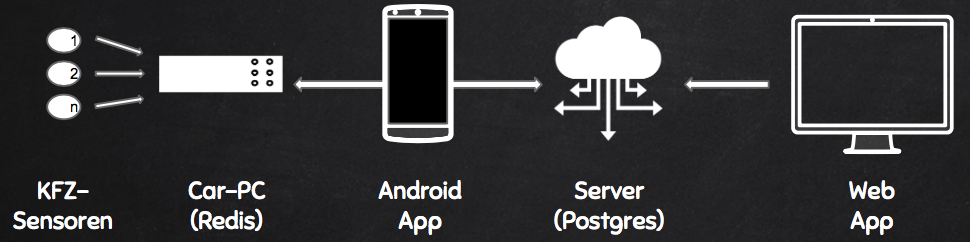
\includegraphics[scale=0.6]{images/konzept}
	\caption{Konzept des BestShift Systems}
	\label{fig:konzept1}
\end{figure}

Abbildung \ref{fig:konzept1} zeigt wie die einzelnen Komponenten des BestShift Systems miteinander interagieren. Das System hat letzendlich folgende Aufgaben zu erfüllen:

\begin{itemize}
	\item Echtzeit Messung und Errechnung der Beschleunigungskräfte, des Schadstoffausstoßes und eines Schaltvorschlags mittels der OBD-II Schnittstelle
	\item Realisierung eines Car-PC für einen größeren Pool an Informationen
	\item Darstellung der Hauptfeatures: Schaltvorschlags, Fahrkomforts und Schadstoßes in einer Android Applikation und einer Web-Applikation
	\item Retrospektive Analyse und Vergleich der Hauptfeatures in der Web-App
	\item Sharing Möglichkeiten für die Analyse einer Fahrt
\end{itemize}

In der folgenden Sektion werden die Probleme beschrieben, welche durch das System gelöst werden sollen und welche Methoden dafür verwendet wurden. Zusätzlich dazu wird auch ein Vergleich zwischen anderen etablierten Konzepten, bzw. umgesetzten Systestemen und dem Projekt BestShift Für eine allgemeine Beschreibung des Projekts, siehe Sektion \ref{sec:projektbestshift}.

\lfoot{Autor: Raphael Simsek}
\subsection{Analyse und Verbesserung des Fahrstils}

Leider kann nicht immer der Fahrlehrer einem Fahrschüler einen nachhaltigen oder wünschenswerten Fahrstil näher bringen, da dies oft auch ein zeitintensiver Prozess ist. Zu diesem Zweck machte man sich Gedanken wie man diese Situation verbessern kann.

Vor der Antragstellung wurde überlegt, ob es bereits bekannte Systeme gibt, um seinen Fahrstil nachhaltig zu verbessern. Man fand dabei heraus, dass es bereits in vielen anderen Bereichen Apps gibt, welche sich das \textit{Sharing}-Prinzip zu Nutze gemacht haben und so äußerst bekannt geworden sind. Eines der bekanntesten österreichischen Beispiele ist das, stetig erweiterte, App-System von Runtastic. \cite{SIMR.CH1-Fahrstil-Analyse.BusinessplanRuntastic}
Nur in Bezug auf das Autofahren konnte kein System, das dieses Prinzip verfolgt, gefunden werden.

\comment{MELD:Was hat das alles konkret mit Analyse und Verbesserung des Fahrstiles zu tun? - Element der Peer-Pressure erklärt und integriert, so besser?}
Zu Beginn des Diplomprojektes gab es also keine Möglichkeiten für verbesserungswillige Autofahrer ihren Fahrstil zu verbessern und dies dann sogar zu teilen. Das Teilen der Fahrstilanalyse trägt aufgrund des \textit{Peer-Pressure}-Effekts dazu bei, dass die Nutzer ihren Fahrstil verbessern, da Sie andere Nutzer überbieten möchten. So versuchen sich die Fahrer dadurch also stetig zu verbessern.
Dies hat unsere Marktumfeldanalyse ergeben, wobei uns besonders auffiel, dass eine Analyse-Funktion für die nachhaltige Verbesserung des Fahrstils nötig wäre. Es wurde für diese Analyse evaluiert, welche Funktionalitäten am wichtigsten sind, wobei diese auch innerhalb der Diplomarbeit realisierbar sein sollten. 
\newline

Eine Analyse des Fahrstils, nach Parametern der Fahrgastbequemlichkeit, ist gar nur bei Sportwagen und Fahrzeugen, die für den Rennbetrieb gedacht sind, verbaut. Hierbei ist anzumerken, dass bei derartigen Fahrzeugen die Funktionalität nicht für das frühzeitige Verbessern des Fahrstils eines Fahrers verwendet wird, sondern für die Optimierung von Rundenzeiten auf einer Rennstrecke oder schier für das Ausreizen des Möglichen.

\begin{figure}[!htb]\centering
	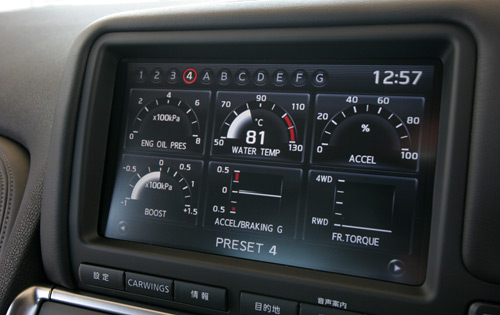
\includegraphics[width=0.6\textwidth]{images/gtrMultifunc}
	\caption{bisherige Analyse Möglichkeiten bei einem Nissan GT-R (R35) \cite{SIMR.CH1-Fahrstil-Analyse.GTRMultifunc}}\label{Fig:imgGTR}
\end{figure}

\newpage
Der bisherige Schaltvorschlag in einem Auto ist, insbesondere bei kostengünstigeren Fahrzeugen, oft äußerst simpel gehalten, wobei ab einer gewissen Drehzahl die darauffolgenden Gänge vorgeschlagen werden oder nur auf den Normzyklus optimiert wird. \cite{SIMR.CH1-Fahrstil-Analyse.Schaltempfehlung} Der Motorwirkungsgrad nach dem Carnot-Prozess, wird dabei aber kaum verwendet. Der Carnot-Prozess beschreibt die Errechnung des \textit{theoretisch möglichen} Motorwirkungsgrad, ohne hinzuziehen von Reibung, Temperatur und anderen natürlichen Einflussgrößen. \cite{SIMR.CH1-Fahrstil-Analyse.CarnotWirkungsgrad} Genauere Ausführungen zu diesem Thema finden Sie im Kaptiel \hyperlink{subsubsection.2.1.2}{Thermodynamik} \todo{fix inter-chapter reference} mehr. 

\begin{figure}[!htb]\centering
	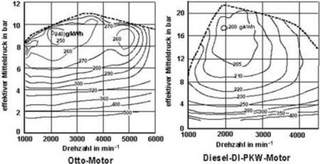
\includegraphics[width=0.6\textwidth]{images/motorkennfeld}
	\caption{Diagramm des Energieverbrauchs beim Otto- und Dieselmotor. Nach rechts ist die Drehzahl aufgespannt, nach oben sieht man die abgegebene Kraft. Man erkennt die niedrigen Verbrauchswerte vor allem bei Volllast. \cite{SIMR.CH1-Fahrstil-Analyse.Motorkennfeld}}\label{Fig:imgMotorkennfeld}
\end{figure}

Eine Live-Messung von \ce{CO2} Werten während der Fahrt ist momentan eine Schätzung, welche durch die Fahrzeughersteller aufgrund der OBD-II Daten durchgeführt und bei sehr wenigen Modellen als Zusatz angezeigt wird. Echte Grenzwerte oder gar eine Analysefunktionalität gibt es in dieser Hinsicht aber nicht. Die \ce{CO2} Werte werden in Zukunft noch weitaus relevanter, weil, wie mein Kollege im folgenden Kapitel ausführlich beschreibt, bis 2020 versucht wird einen Durschnittsaustoss von 95 g/km zu erzielen. \cite{SIMR.CH1-Fahrstil_Analyse.EUVerordCO2}

Weil aber besonders Fahranfänger und Fahrer die eben genannte Analysefunktionalität möglicherweise gerne nutzen würden, wurde ebenfalls evaluiert ob es diese Möglichkeiten durch Zubehör bereits gibt.

Bei der Evaluierung wurde ein Projekt entdeckt, welches die gelieferten Daten nur live per Computer auslesbar macht, die Programmierung ist dabei so anders dass man dies nicht auf Android portieren könnte. Das Projekt ist außerdem weitaus teurer als angedacht (Low Budget CarPC: €300-350,-, gewünschtes Budget: < €100,-) Daher wurden Überlegungen angestellt, wie man die Idee eines solchen Projektes massentauglicher machen kann und dabei trotz des niedrigeren Preises dem Nutzer ein wünschenswertes Erlebnis bieten kann. \cite{SIMR.CH1-Fahrstil-Analyse.LowBudgetCarPC} Dieses Projekt hat uns also geholfen in der Defintionsphase des Projektes Anpassungen vorzunehmen, da es bereits einen Maßstab gab, was im Bereich des Möglichen liegt.

Die Möglichkeit einer Analyse konnte aber bei der Evaluierung bei keiner der konkurrierenden Echtzeit-Anzeigen (wie. z.B. Torque Pro \cite{SIMR.CH1-Fahrstil-Analyse.TorquePro}) erkannt werden. 

\begin{figure}[!htb]\centering
	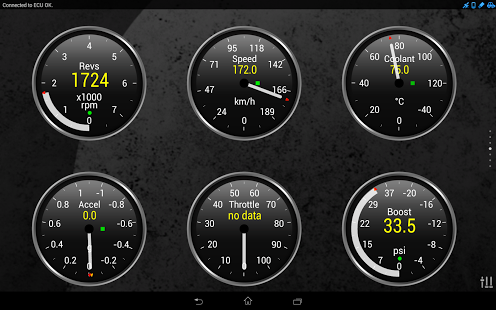
\includegraphics[width=0.6\textwidth]{images/torquePro}
	\caption{Möglichkeiten mit der kostenpflichtigen Torque Pro App und der OBD Schnittstelle \cite{SIMR.CH1-Fahrstil-Analyse.TorquePro}}\label{Fig:imgGTR}
\end{figure}

Gerade diese Funktionalität würde aber von Fahranfängern benötigt werden um frühzeitig und selbstständig Fehler ihres Fahrstils zu erkennen und auszubessern zu können. Insbesondere konnten wir, unter anderem anhand unserer Erfahrungen, feststellen, dass das Schalten und das gleichmäßige und verbrauchsarme Fahren für viele Fahranfänger eine Herausforderung darstellt. Durch eine Analyse Funktion könnten motivierte Fahranfänger Anfangsschwieriegkeiten schneller ablegen und die schlechten Angewohnheiten würden sich nicht im  Gedächtnis eines Fahranfängers verankern, sondern es würden sich nur positive Charakteristika gemerkt werden. \comment{JOSC: Definiere bitte positive und schlechte Angewohnheiten oder formulier um - so?} 

Eine Analysefunktion in Form einer Webapplikation ist also insbesondere für die Lernkurve bei einem noch ungeübten Kraftfahrzeug-Lenker von großem Vorteil, da diese oft noch nach dem Erhalt des Führerscheins unsicher bezüglich ihres Fahrstils sind und des öfteren wiederholt die selben, genannten, Fehler unbemerkt begehen.

Andererseits kann solch eine Funktionalität auch von großer Hilfe als lernunterstützendes Medium sein, da momentan ein Fahrschüler nach seiner Fahrstunde nur ein subjektives Feedback seines Fahrlehrers bekommt. Wie ließe sich eine solche Lernunterstützung also umsetzen?
Man könnte dem Fahrschüler am Ende der Fahrstunde eine faktenbasierte Übersicht über seine Leistung während der Fahrstunde geben, welche er dann auch mitnehmen kann. Mit dieser Information kann sich der Fahrschüler ohne Fahrlehrer mit der App selbst im Auto auf abgesperrtem Grund verbessern um sich so auf die nächste Fahrstunde vorzubereiten.

Ein geübter, umweltfreundlicher Fahrer könnte mit der passenden Analysefunktion auch den produzierten \ce{CO2} Ausstoß messen und so seinen Bleifuß besser regulieren.
\clearpage % DO NOT REMOVE

\subsection{Umweltbelastung durch \ce{CO2} Ausstoß}
\lfoot{Autor: Hüseyin Bozkurt}
\label{subsec:umweltbelastungco2}

\subsubsection{Definition und Entstehung}
Kohlenstoffdioxid (\ce{CO2}) ist ein unsichtbares, geruchsloses Gas bestehend aus einem Kohlenstoff und zwei Sauerstoff-Atomen. 
In jedem Stoffwechselprozess spielt Kohlenstoffdioxid eine wichtige Rolle, da beispielsweise der Mensch \ce{CO2} ausatmet. 
Bei vielen Energiegewinnungsverfahren werden durch Verbrennung Energien freigesetzt, die als Nebenprodukt Kohlenstoff produzieren. 
In der freien Luft verbinden sich diese Kohlenstoffpartikel mit Sauerstoff zu \ce{CO2}, dieses ist
Reaktionsträge und besitzt keine giftige Eigenschaft. 
Das Problem mit den Unmengen an ausgestoßenem \ce{CO2} ist, dass sein massives Vorkommen die Atmosphäre beschädigt.

Alle Fahrzeuge, die fossile Brennstoffe als Energiequelle nutzen 
(wie zum Beispiel Diesel, Flüssiggas, Benzin und auch Biotreibstoff), erzeugen Kohlenstoff als Abgas. 
Indem der Motor den Kraftstoff zusammen mit Luftsauerstoff verbrennt, gelangt das \ce{CO2} über die Abgasanlage in die Atmosphäre. 
Eine effektive Methode zur Beseitigung der Kohlenstoffpartikel gibt es zurzeit nicht. 
Der benutzte Kraftstoff bestimmt, wie viel \ce{CO2} bei der Verbrennung als Nebenprodukt entsteht.
Beispielsweise entsteht bei der Verbrennung von einem Liter Diesel mehr Kohlenstoffdioxid, als bei einem Liter Benzin.
Der Kraftstoffverbrauch eines Kraftfahrzeugs und sein \ce{CO2}-Ausstoß stehen daher in enger Verbindung.
Demnach existieren Werte, die man als Grenze für den Verbrauch festlegen kann. 
Heutzutage sprichen wir von der Einheit Gramm pro Kilometer [g/km] als normierte Verbrauchsmessung.
Der Lenker eines PKW hat Einfluss auf seinen \ce{CO2}-Ausstoß, indem dieser bei starken und überflüssigen Beschleunigungsmanövern
zu diesem Zeitpunkt mehr Schadstoffe produziert als nötig.
Mit diesem Diplomprojekt, wollen wir Fahrenden ein Werkzeug anbieten, damit sie ihren \ce{CO2}-Ausstoß während und nach der Fahrt
einschätzen können. Damit haben sie die Möglichkeit ihre Fahrweise in Hinblick auf den \ce{CO2}-Ausstoß zu verbessern.

\clearpage

\subsubsection{Treibhauseffekt}
\ce{CO2} gilt als eines der häufigsten Treibhausgase.
Das Kohlenstoffdioxid steigt bis zur Atmosphäre auf und bildet dort eine \textit{Mauer}.
Sonnenstrahlen können zwar ohne weiteres durch, doch nicht so leicht wieder raus. Die Sonnenstrahlen,
die von der Erdoberfläche wieder zurück in den Weltraum reflektiert werden sollten, werden von der Erdatmosphäre zurück auf die Erde geworfen und erzeugen
damit eine höhere Durchschnittstemperatur.
Der Treibhauseffekt gilt als eine der Hauptursachen für den Klimawandel, welcher drastische Folgen für Natur, Tiere und Menschen hat. 
Zu viel \ce{CO2} in der Atmosphäre bringt unter anderem das Abschmelzen von Gletschern, 
den Anstieg der Meerestemperatur, den Anstieg des Meeresspiegels, 
Aussterben von Pflanzen und Tieren und Wetterphänomene wie zum Beispiel sehr warme Winter, Stürme etc.

\begin{figure}[!htb]\centering
	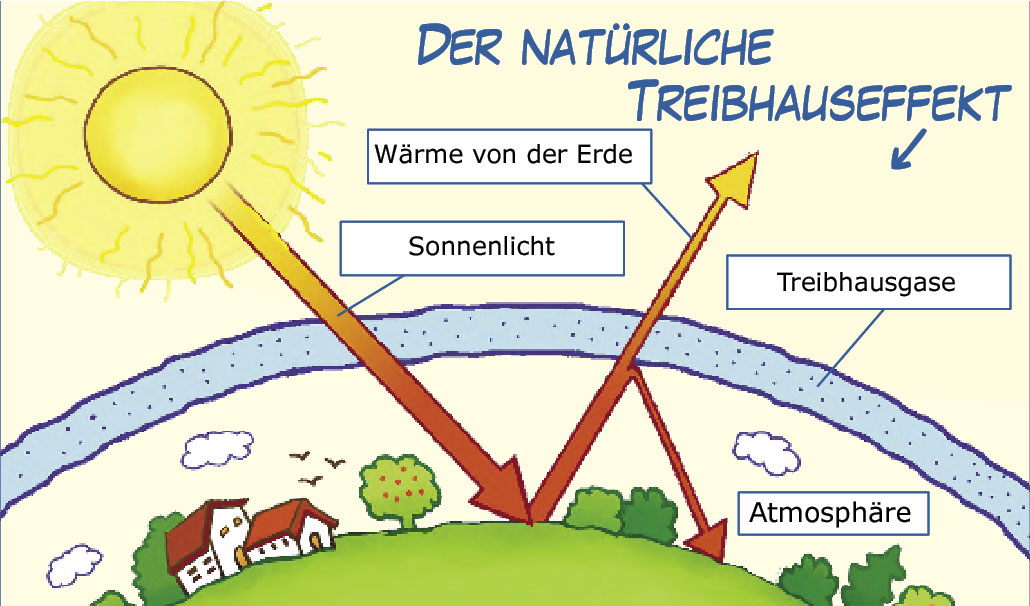
\includegraphics[width=0.6\textwidth]{images/treibhaus1}
	\caption{Der Treibhauseffekt \cite{BOZH.ch1-co2-umwelt.treibhaus1}}
\end{figure}
 
\subsubsection{Das Kyoto-Protokoll}
Im Rahmen des Kyoto-Protokolls haben sich viele westliche Staaten zu einer Reduktion der Treibhausgase verpflichtet. 
Dieses Protokoll war der Startschuss für die Suche nach erneuerbaren Energien. 
Anfang 2015 sind Gesetzesregelungen in Kraft getreten, die den Durchschnittsverbrauch eines PKW auf 130g/\ce{CO2} pro Kilometer limitierten. 
Bis 2020 soll dieses Limit auf 95g/CO2 pro Kilometer herunter gesetzt werden.

\clearpage
\lfoot{Autor: Faiku Fitim}
\subsection{Das Projekt BestShift}

BestShift ist ein Projekt, welches dem Fahrer Informationen während- und nach der Fahrt bieten soll. 
Dazu werden in unterschiedlichen Teilen des Projektes 
diverse einzelne Komponenten einer hybriden Android Applikation und einer Hardware Schnittstelle für das ODB-II 
Interface entwickelt. 
Eine zusätzliche Web-App ermöglicht es, Fahrten retrospektiv zu betrachten und während der Fahrt gesammelte Daten innerhalb eines sozialen Netzwerkes zu teilen.
 

Für die Smartphone Applikation wird ein Android Framework verwendet, 
während die Hardware aus einem Single Board Computer (SBC) bestehen soll. 
Mittels einem ODB-II zu Bluetooth Chip (ELM237) und Python, 
werden Daten aus dem Motormanagement sowie eigene Sensordaten, welche in einem selbstgemachtem Car-PC eingebaut sind,
gesammelt und aufbereitet. 
Die gesammelten Daten können dann von dem Smartphone aus in die Cloud geladen werden, welche dann durch unsere
Webapplikation genauer inspiziert werden können.

In diesem Projekt wird eine Applikation für das mobile Betriebssystem Android implementiert, 
die dem Fahrer eines KFZ während der Fahrt Informationen zu Fahrgastbequemlichkeit und verbrauchseffizienter Fahrweise gibt. 
Dazu werden Daten aus dem Motormanagement verwendet. 
Für weitere benötigte Daten (z.B. Beschleunigungswerte) werden zusätzliche externe Sensoren in einem portablen CarPC integriert. 
Das Herzstück des Projektes ist aber die Webapplikation, die die Retrospektive Fahrtenanalyse und eine Social Media implentierung beinhaltet.
Diese Webapplikation wird die Möglichkeit bieten, die gesammelten Daten aller gespeicherten 
Fahrten für spätere Analysen graphisch einfach aufbereitet anzuzeigen. 
Die einzelnen Messwerte sollen dabei mit geographischen Informationen verknüpft werden, 
um dem Fahrer zum Beispiel zu zeigen, welche Stellen der Strecke besonders verbrauchsintensiv oder unbequem für den Fahrgast waren. 

Als weitere Funktion soll die Applikation aus den ermittelten Daten dem Fahrer den 
momentan am energieeffizientesten oder leistungsstärksten Gang vorschlagen können.
\clearpage % DO NOT REMOVE